\chapter{Thermodynamic Basis} \label{chap:thermo}

The laws that govern all material systems can be expressed in two seemingly simple statements of Rudolf Clausius - \emph{``Die Energie der Welt ist konstant. Die Entropie der Welt strebt einem Maximum zu.''} and yet thermodynamics has drawn the attention of many great scientists including Maxwell, Boltzmann, Planck and  Mach. Physicist Arnold Sommerfeld accounted his experience of thermodynamics as \emph{``Thermodynamics is a funny subject. The first time you go through it, you don't understand it at all. The second time you go through it, you think you understand it, except for one or two small points. The third time you go through it, you know you don't understand it, but by that time you are so used to it, it doesn't bother you any more''}. A number of definitions and laws of thermodynamics form the basis of equilibrium thermodynamics and the Gibbs energy models and equations play a key role in the structure of the equilibrium solver.

%==============================================================================================================================
%															Definitions
%==============================================================================================================================
%\section{Definitions}
%

%==============================================================================================================================
%														Laws of Thermodynamics
%==============================================================================================================================
\section{Fundamental Laws of Thermodynamics}
	The statements of Rudolf Clausius are now known as the \emph{First and Second Laws of Thermodynamics}. Before looking at these laws, the basic definitions used in subsequent sections are reviewed for clarity. A \emph{thermodynamic system} is a portion of the universe with a perimeter defined by real or imaginary boundaries and usually consists of many chemical components whose thermodynamic behaviour can be analysed. For example, the volume element shown in figure~\ref{fig:system} can be treated as a thermodynamic system. A system that may exchange matter with its system boundary is called \emph{open} while a system that can only exchange energy and not matter is called \emph{closed}. The term \emph{isolated} is used for a system that is cut off from the surroundings and can neither exchange matter nor energy. In material thermodynamics, the system is often treated as closed, notable exceptions being chemical reactors where reactants and products continuously flow in and out of the system.
 	\begin{figure}[htb]
		\centering
		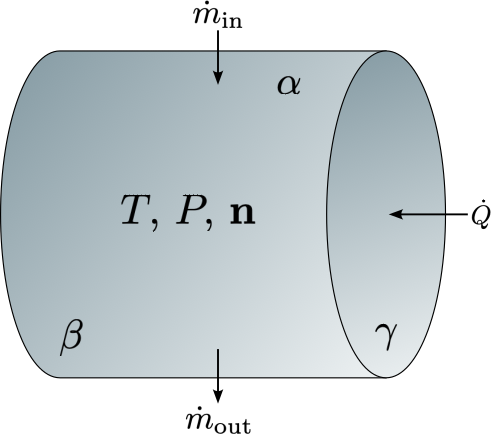
\includegraphics[width=0.45\textwidth]{figures/chapter-3/system.png}
		\caption{Volume element of a general thermodynamic system with mass flow of chemical components $\dot{m}$ and heat flux $\dot{Q}$. The Greek letters indicate presence of separate phases.}
		\label{fig:system}
	\end{figure}

	A thermodynamic system can be described macroscopically using \emph{state variables}, which are represented by measurable macroscopic quantities such as temperature, pressure, volume, amounts of different substances, etc. \emph{Intensive variables} (e.g. temperature and pressure)  are independent of the amount of matter in the system  while  \emph{extensive variables} (e.g. volume and total internal energy) are dependent on the mass of the system.  With a change in the internal variables, the system undergoes a change in state. If a system can be restored to the original condition without any change in the state of the surroundings, the process through which the state of the system was changes is described as a \emph{reversible process}. However, all real processes are \emph{irreversible processes}, that is, the system cannot be recycled.

	Thermodynamics concerns the state of a system as it interacts with its surroundings and is based on two physical laws: the first and second laws of thermodynamics. The first law of thermodynamics describes those interactions, which can involve exchanges of any combinations of heat, work, and mass, while the second law of thermodynamics governs the evolution of state inside the system. Together, the two laws integrate the external and internal parts of the system.

	\subsection{First law of thermodynamics}
	The first statement of Clausius and what is now known as the first law of thermodynamics expresses the conservation of energy\footnote{Considering Einstein's mass-energy equivalency, the classical first law can be modified to state that mass and energy together are constant. However, since we are considering chemical equilibrium and not dealing with nuclear reactions, the classical form of first law applies.} and is formulated as follows:

		\hangindent=\parindent \emph{Energy cannot be created or destroyed, and the energy increase of a system ($dU$) equals the sum of the heat absorbed from the surroundings ($dQ$) and the work ($dW$) done by the surroundings on the system.}

	\noindent Mathematically, for an open system, the first law can be expressed as:
	\begin{equation}\label{eqn:flot}
		dU = dQ + dW + \sum H_i dN_i,
	\end{equation}
	where $dN_i$ denotes the amount of component $i$ exchanged with the surroundings and $H_i$ is the unit energy of component $i$ in the surroundings, and the summation is for all the independent components in the system. Since the systems of interest in thermodynamics of materials are closed, there is no exchange of matter between the system and the surroundings and the first law of thermodynamics takes the following form:
	\begin{equation}\label{eqn:flot1}
		dU = dQ + dW,
	\end{equation}
	where both $dQ$ and $dW$ depend on the thermodynamic process and hence do not qualify as state functions.

	\subsection{Second law of thermodynamics}
	In 1850, Clausius formulated a criterion for the direction of spontaneous processes and called it \emph{entropy}. His second statement translates to entropy of the universe tends to maximum and is now known as the second law of thermodynamics. Formally, the second law states that:

	\hangindent=\parindent \emph{For an internal process to take place spontaneously, or irreversibly, the change in entropy of the system ($dS$) must be positive.}

	\noindent In mathematical form, the second law can be formulated as:
	\begin{equation}\label{eqn:slot}
		dS = dS_\text{sys} + dS_\text{surr} \geq 0,
	\end{equation}
	where the $S_\text{sys}$ and $S_\text{surr}$ represents the entropy of the system and surroundings respectively.
	In the course of a reversible, isothermal process, the entropy change of the system $dS_\text{sys}$   can be defined as the heat exchange divided by temperature:
	\begin{equation}\label{eqn:slotrev}
		dS_\text{sys} = \frac{dQ}{T}.
	\end{equation}

	\subsection{Third law of thermodynamics}
	The third law of thermodynamics allows expressing the absolute value of the entropy in contrast to the internal energy by assigning an entropy equal to zero at \SI{0}{\kelvin} for any pure compound in stable and perfectly crystalline state.

%==============================================================================================================================
%												Enthalpy, and Helmholtz and Gibbs Energies
%==============================================================================================================================
\section{Enthalpy, and Helmholtz and Gibbs Energies}
		Three important state functions of great practical importance in thermodynamics are the \emph{enthalpy} $H$, \emph{Helmholtz energy} $F$, and \emph{Gibbs energy} $G$. Enthalpy changes are of importance in calorimetry experiments as they can be directly measured while Helmholtz and Gibbs energies are used in defining chemical equilibrium conditions.

		The enthalpy of a thermodynamic system is an extensive property defined as:
		\begin{equation}
			H = U + PV,
		\end{equation}
		where $U$ denotes the internal energy, $P$ denotes the pressure the system is at and $V$ represents the volume of the system.

		The Helmholtz energy of a thermodynamic system is defined as:
		\begin{equation}
			F = U - TS,
		\end{equation}
		where, $T$ denotes the absolute temperature of the system and $S$ represents the entropy of the system.

		The Gibbs energy of a thermodynamic system is defined as:
		\begin{equation}
			G = H - TS.
		\end{equation}

		The equilibrium criterion can be derived in terms of Helmholtz and Gibbs energies. According to the second law of thermodynamics, a spontaneous irreversible process must be accompanied by an overall positive change of entropy, i.e.:
		\begin{equation}
			dS_\text{sys} + dS_\text{surr} > 0.
		\end{equation}
		For a closed system in thermal and mechanical equilibrium but not in chemical equilibrium which acquires an infinitesimal quantity of heat from the surroundings:
		\begin{equation}
			dS_\text{surr} = -\frac{dQ_\text{sys}}{T},
		\end{equation}
		where it is assumed that the mass of the surroundings is large enough so that addition/removal of the heat does not cause a perceptible change in temperature. Thus,
		\begin{equation}
			{dQ_\text{sys}} - T dS_\text{sys}  < 0.
		\end{equation}

		Assuming that the heat exchange causes an infinitesimal change in the internal energy of the system by an amount $dU_\text{sys}$, according to the first law of thermodynamics,
		\begin{equation}
			{dU_\text{sys}} = {dQ_\text{sys}} + {dW_\text{sys}}.
		\end{equation}

		For a closed, isobaric system the work is purely due to the change in the volume of the system and the following relationship is obtained:
		\begin{equation}
			{dU_\text{sys}} + P{dV_\text{sys}} - T{dS_\text{sys}} < 0.
		\end{equation}

		If both the temperature and volume were held constant, the above inequality becomes:
		\begin{equation}
			d{U_\text{sys} - TS_\text{sys} } < 0.
		\end{equation}

		Since the terms within the parentheses denote the Helmholtz energy, we obtain the criterion for spontaneous change of isothermal, isochoric system, which is expressed as:
		\begin{equation}
			d{F_\text{sys} } < 0
		\end{equation}

		Similarly, if the temperature and pressure were held constant, the inequality becomes:
		\begin{equation}
			d{U_\text{sys} + PV_\text{sys} - TS_\text{sys} } < 0.
		\end{equation}

		The terms inside the parentheses denote the Gibbs energy and subsequently yield the criterion for spontaneous change of an isothermal, isobaric system:
		\begin{equation}
			d{G_\text{sys} } < 0.
		\end{equation}

		Thus, for the equilibrium of a closed system at constant temperature and volume, it is necessary and sufficient that the Helmholtz energy of the system is at minimum and equivalently, the Gibbs energy of the system must be at minimum for equilibrium in systems at constant temperature and pressure. In equilibrium thermodynamics, Gibbs energy is often preferred over Helmholtz energy since controlling pressure is easier than controlling volume during experiments. It must be emphasised that thermodynamic properties are fundamentally concerned with relative changes, a property that is often exploited in computations.

%==============================================================================================================================
%												Gibbs Energy and Chemical Potential
%==============================================================================================================================
\section{Gibbs Energy and Chemical Potential}
	Of particular interest in description of  thermodynamic equilibrium are the quantities named \emph{potentials}. A system is in thermodynamic equilibrium when it is simultaneously in thermal, mechanical, electrical and chemical equilibrium. This also refers to the state where there are no unbalanced potentials within the system. J.W. Gibbs used the term \emph{thermodynamic potential} to represent all the relevant system potentials to characterise the conditions of thermodynamic equilibrium \cite{Gibbs:1878aa}. Thermodynamic equilibrium calculations are based on the principle that the potential for each component must be uniform throughout the system at thermodynamic equilibrium. This section and the following describe the relation between Gibbs energy and chemical potentials and their use in computing thermodynamic equilibrium.

	The Gibbs energy, $G_{i}$ [\si{\joule \per \mole}], of a pure species  $i$ is defined as \cite{Zemansky81}:
	\begin{equation} \label{eqn:Gibbs_der1}
			G_{i} = \Delta H_{i} - TS_{i},
	\end{equation}
	where T [\si{\kelvin}] is the absolute temperature, $\Delta H_{i}$ [\si{\joule \per \mole}] and $S_{i}$ [\si{\joule \per \mole \per \kelvin}] represent the enthalpy and absolute entropy of species $i$ in phase $\phi$ respectively. Since thermodynamic quantities are relative in nature, equation ~\eqref{eqn:Gibbs_der1} can be expanded as:
	\begin{equation} \label{eqn:Gibbs_der2}
			G_{i} = \left(\Delta H_{i}^\circ + \int_{T_0}^{T} C_{p,i}dT \right) - T\left( S_{i}^\circ  + \int_{T_0}^{T} \frac{C_{p,i}}{T}dT \right) + \int_{P_0}^{P} V_i dP,
	\end{equation}
	where $\Delta H_{i^\circ}$ [\si{\joule \per \mole}] and $S_{i^\circ}$ [\si{\joule \per \mole \per \kelvin}] are the standard enthalpy of formation and entropy respectively at standard temperature ($T_0 = 298.15$ \si{\kelvin}) and pressure ($P_0 = 1$ \si{atm}). The superscript / subscript $\circ$ represents a quantity at standard temperature and pressure, a notation that is used hereafter. $C_{p,i}$ [\si{\joule \per \mole \per \kelvin}]  denotes the molar heat capacity at constant pressure, $P$ [\si{atm}] is the absolute pressure and $V_i$ [\si{\meter \cubed \per \mole}] denotes the molar volume. For an ideal gas, from the gas law, the last term in equation~\eqref{eqn:Gibbs_der2} can be written as $RT \ln{\left(P/P_0\right)}$, where $R = 8.314462$ [\si{\joule \per \mole \per \kelvin}] is the ideal gas constant. For a pure ideal gas species $i$, the standard Gibbs energy is:
	\begin{equation} \label{eqn:Gibbs_der_id}
			G_{i} = \left(\Delta H_{i}^\circ + \int_{T_0}^{T} C_{p,i}dT \right) - T\left( S_{i}^\circ  + \int_{T_0}^{T} \frac{C_{p,i}}.{T}dT  - R \ln{\left(\frac{P}{P_0}\right)}\right).
	\end{equation}

	The fact that Gibbs energies are relative quantities and can be numerically adjusted as long as the elemental differences are preserved is of practical importance and is often used in thermodynamic equilibrium calculation. Chemical potential of species $i$ in phase $\lambda$, $\mu_{i(\lambda)}$ [\si{\joule \per \mole}], is a measure of the change of the Gibbs energy of the system by the introduction of species $i$ and incorporates  the reference Gibbs energy of pure species, $g_{i}^\circ$, and the entropic contribution due to mixing as a function of its mole fraction. Mathematically, the chemical potential of a species $i$ is defined as \cite{Zemansky81}:
    	\begin{equation}\label{eq:mu_def}
        		\mu_{i} = {\left (\frac{\partial G_\text{sys}}{\partial n_{i}} \right )}_{T,P,n_{j \neq i}}.
    	\end{equation}

	For the species of a phase with only ideal mixing, the chemical potential is generally given as:
    	\begin{equation}
        		\mu_{i} = g_{i}^\circ + \ln x_{i}.
    	\end{equation}

	For non-ideal solution phases, the chemical potential also includes the partial molar excess Gibbs energy of mixing, $g_{i}^{ex}$ [\si{\joule \per \mole}], to account for non-ideal mixing as follows:
    	\begin{equation}\label{eq:mu_ex}
        		\mu_{i} = \mu_{i}^\circ + \ln x_{i} + \mu_{i}^{ex}.
    	\end{equation}

    	While the chemical potential of stoichiometric phases does not include a composition dependent term, the partial molar excess Gibbs energies of mixing for non-ideal solution models depend on the mixing model employed. Some of these models include the Modified Quasichemical Model \cite{Pelton00,Pelton01,Chartrand01,Pelton01b,Lambotte11}, the Compound Energy Formalism \cite{Hillert01}, etc.

	The integral Gibbs energy of a multicomponent, multiphase system is represented as:
	\begin{equation}\label{eqn:integralGibbs1}
        		G_\text{sys} = RT \left ( \sum_{\phi=1}^{\Phi} n_{\phi} \sum_{i=1}^{N_{\phi}}x_{i}\tilde{\mu}_i \right ),
    	\end{equation}
	where $R$ [\si{\joule \per \mole \per \kelvin}] is the ideal gas constant, $T$ [\si{\kelvin}] is the absolute temperature, $N_{\phi}$ denotes the number of species in phase $\phi$ of which there can be a maximum of $\Phi$ and $x_{i}$ represents the mole fraction of species $i$. For convenience, the Gibbs energy is often split into separates contributions from solution and stoichiometric phases as follows:
    	\begin{equation}\label{eqn:integralGibbs}
        		G_\text{sys} = RT \left ( \sum_{\lambda=1}^{\Lambda} n_{\lambda} \sum_{i=1}^{N_{\lambda}}x_{i}\tilde{\mu}_i + \sum_{\omega=1}^{\Omega} n_{\omega} \tilde{\mu}_{\omega} \right ),
    	\end{equation}
    	$N_{\lambda}$ denotes the number of species in the solution phase $\lambda$ and $x_{i}$ represents the mole fraction of species $i$ in solution phase $\lambda$. $\Lambda$ and $\Omega$ represent the number of stable solution phases and stoichiometric phases, respectively, and the number of moles of the solution phase $\lambda$ and stoichiometric phase $\omega$ are denoted by $n_\lambda$ and $n_\omega$ [\si{\mole}], respectively. $\tilde{\mu_i}$ represents the dimensionless form of the chemical potential of species $i$ and is given as $\tilde{\mu}_i = \mu_i / RT$\footnote{The dimensionless form $\tilde{\mu}_i$ has been used here as it is the preferred form in computational implementations.}. Finally, $\tilde{\mu}_i$ and $\tilde{\mu}_\omega$ represent the dimensionless chemical potential of species $i$ in solution phase $\lambda$ and stoichiometric phase $\omega$ respectively.

	The Gibbs energy of  the system can also be expressed in terms of the element potentials, $\Gamma_j$ [\si{\joule \per \mole}], and the number of moles, $b_j$ [\si{\joule}], of the system components. Mathematically, this can be expressed as:
	\begin{equation}\label{eq:elempot}
        		G_\text{sys} = \sum_{j=1}^{C} \Gamma_j b_j,
    	\end{equation}
	where $C$ denotes the number of system components which is normally the number of elements in the system. The mixing models used in materials modelling are briefly described in the following section.

	\subsection{Excess mixing models for Gibbs energy}
	A number of different models for excess mixing component of Gibbs energy have been proposed in literature. The different models are suitable for different materials, for example the Compound Energy Formalism (CEF) is often used for \ce{UO2} fuels while the Modified Quasichemical Model (MQM) is the state of the art model used to describe molten salts, which are of prime interest in the development of MSRs. However, only the relevant equations for some of the most commonly used models are shown here.
	\begin{enumerate}
	\item \textbf{Substitutional solution models}\\
	The regular solution model is a quantitative explanation of non-ideal behaviour. The model assumes that the entropy of mixing is the same as ideal mixing but that the enthalpy of mixing is not zero. A number of different regular solution models have been proposed, the most commonly used ones being based on Kohler-Toop and Redlich-Kister-Muggiano interpolation schemes \cite{Lukas07}.
		\begin{itemize}
			\item \textbf{Kohler-Toop Interpolation}
			\begin{equation}
				g_{\lambda}^\text{ex} = \sum_{z=1}^Z \phi_z (x_1^{d_1} x_2^{d_2} x_3^{d_3} ).
			\end{equation}
			\item \textbf{Redlich-Kister-Muggiano Interpolation}
			\begin{equation}
				g_{\lambda}^\text{ex} = \sum_{z=1}^Z x_j x_k \sum_{\nu = 0} {^\nu}L_{j}.
			\end{equation}
			\end{itemize}
	\item \textbf{Compound Energy Formalism (CEF)} \\
	Compound Energy Formalism is a multi-sublattice model proposed by Hillert \cite{Hillert01} for an adequate description of the properties of solution phases with sublattices. The molar Gibbs energy, $g_{\lambda}$, of solution phase $\lambda$ based on the CEF model is generally given as:
	\begin{equation}\label{eq:g_lambda}
	g_{\lambda} = \sum_{i=1}^{N_{\lambda}} g_{i}^{\circ} \prod _{s=1}^{N_s} y_{i(s)} + RT\left( \sum_{s=1}^{N_s} a_s \sum_{c=1}^{N_c}   y_{c(s)} \mathrm{ln} (y_{c(s)}) \right) + g_{\lambda}^\text{ex},
	\end{equation}
	where $g_{i}^{\circ}$ is the standard molar Gibbs energy of the pure component $i$,
$y_{i(s)}$ represents the site fraction on sublattice $s$ corresponding to component $i$, $N_{\lambda}$ and
$N_s$ denote the number of components and number of sublattices in solution phase $\lambda$, respectively.
The ideal gas constant is represented by $R$, the absolute temperature by $T$, the stoichiometry
coefficient for sublattice $s$ is represented by $a_s$, the number of constituents on sublattice $s$ is $N_c$
and the site fraction of constituent $c$ on sublattice $s$ is $y_{c(s)}$.  It is to be understood that $y_{i(s)}$
refers to the site fraction of  constituent $c$ associated with component $i$ on sublattice $s$ and is thus
related to $y_{c(s)}$.  Finally, the molar excess Gibbs energy of mixing of solution phase $\lambda$ is
$g_{\lambda}^\text{ex}$ and is given as:
\begin{equation}
	\label{eq:g_ex}
	g_{\lambda}^\text{ex} = 	 \sum_{p=1}^{N_p} \left( \prod_{m=1} y_{m(s)}  \right)   \sum_{z=0}^{N_z} {^zL_{j,k}} (y_j - y_k)^{z},
\end{equation}
where $N_p$ denotes the number of excess mixing parameters (note: $N_p \ge N_s$), $y_m$ is the site fraction of constituent $m$ corresponding to mixing parameter $p$, $N_z$ is the number of terms corresponding to parameter $p$,  and ${^zL_{j,k}}$ is the $z$th order mixing parameter. A detailed description of CEF can be found in the paper by Hillert \cite{Hillert01}.
	\item \textbf{Modified Quasichemical Model (MQM)} \\
	The Modified Quasichemical Model (MQM) in the quadruplet approximation is the most generalised thermodynamic model for treating Short Range Ordering (SRO). MQM is fundamentally different than other thermodynamic models in that the focus is not on the mixing of chemical species or constituents on a lattice, but rather the mixing of species as quadruplets to capture SRO of both First Nearest Neighbour (FNN) and Second Nearest Neighbour (SNN) in liquid or solid solutions. The details of evolution of MQM from pair approximation for species mixing on only one sublattice to the current quadruplet approximation are provided by Pelton \textit{et al.} \cite{Pelton00,Pelton01,Chartrand01,Pelton01b}.

        For a solution with two sublattices, which is occupied only by a single species on the second sublattice, the SNN pair exchange can be written as:
            \begin{equation} \label{SNNPairExchange1}
	            (A-[X]-A) + (B-[X]-B) = 2(A-[X]-B); \Delta g_{AB/X},
            \end{equation}
        where $\Delta g_{AB/X}$ is the non-configurational Gibbs energy for the formation of 2 mol of $(A-[X]-B)$ pairs. Similarly, when there is a single species on the first sublattice, the formation of SNN pairs is captured via:
            \begin{equation} \label{SNNPairExchange2}
	            (X-[A]-X) + (Y-[A]-Y) = 2(X-[A]-Y); \Delta g_{A/XY}
            \end{equation}
        where $\Delta g_{A/XY}$ is the non-configurational Gibbs energy for the formation of 2 mol of $(X-[A]-Y)$ pairs.
        Among the FNN pairs, the following exchange reaction is considered:
            \begin{equation} \label{FNNPairExchange}
	            (A-X) + (B-Y) = (A-Y) + (B-X); \Delta g_{A/XY}^\text{exchange}
            \end{equation}
        where $\Delta g_{A/XY}^\text{exchange}$ is the non-configurational Gibbs energy.
        Let $n_i \; (i=A,B,...,X,Y...)$ represent the number of moles of species $i$, $n_{i/j}$ be the number of moles of FNN ($(i - j)$) pairs, and $n_{ij/kl}$ be the number of moles of the quadruplets. The relationship between the foregoing terms is \cite{Pelton01b}
        \begin{gather}\label{EqMassBalance1}
	       Z_A n_A  = 2n_{A_2/X_2} + 2n_{A_2/Y_2} + 2n_{A_2/XY} + n_{AB/X_2} + n_{AB/Y_2} + n_{AB/XY} + \cdots, \\
	       Z_X n_X  = 2n_{A_2/X_2} + 2n_{B_2/X_2} + 2n_{AB/X_2} + n_{A_2/XY} + n_{B_2/XY} + n_{AB/XY} + \cdots,
        \end{gather}
        where $Z_A$ and $Z_B$ are the coordination numbers for A and B, respectively. A generic statement for a multi-component system is:
  	\begin{equation}
		Z_i n_i = 2n_{ii} + \sum_{j \ne i} n_{ij}.
         \end{equation}
        The mole fractions then follow:
        \begin{gather} \label{EqMoleFraction}
            x_{i} = \frac{n_{i}}{\sum n_j}, \\
            x_{k} = \frac{n_{k}}{\sum n_l},
        \end{gather}
        where the indices $i$ and $j$ refer to the species on first sublattice while the indices $k$ and $l$ refer to the species on second sublattice.
        The FNN pair fractions and quadruplet fractions are defined as:
        \begin{gather} \label{EqPairFraction}
            x_{i/k} = \frac{n_{i/k}}{\sum_j \sum_l n_{j/l}}, \\
            x_{ij/kl} = \frac{n_{ij/kl}}{\sum n_{ij/kl}}.
        \end{gather}
        Another useful term is the coordination equivalent fraction, which is
            \begin{gather} \label{EqCoordEqFraction}
	            y_i = \frac{Z_i n_i}{\sum Z_j n_j}, \\
	            y_k = \frac{Z_k n_k}{\sum Z_l n_l}.
            \end{gather}
	\end{enumerate}
	Omitting detailed description of the derivation of the model, the simplest form of MQM for binary solutions can be written as:
	\begin{equation} \label{EqGibbsMQM1}
		G_{\lambda} = (n_A g_A^\circ + n_B g_B^\circ) - T\Delta S^\text{config} + \frac{n_{AB} \Delta g_{AB}}{2}
	\end{equation}
	where $g_i^\circ$ is the reference molar Gibbs energy of pure $i$ (computed from a database), $T$ is the absolute temperature, and $\Delta S^\text{config}$ is the configurational entropy, given by:
	\begin{multline} \label{EqConfigEntropy}
		\Delta S^\text{config} = -R\left( n_A \ln(x_A) + n_B \ln(x_B) \right . \\
		+ \left . n_{AA}\textrm{ln}(x_{AA}/y_A^2) + n_{BB}\ln(x_{BB}/y_B^2) +n_{AB}\ln(x_{AB}/(2y_A y_B)) \right)
	\end{multline}

	MQM is of particular interest in this work because it is the preferred model for thermodynamic modelling of molten salts. However, from the computational perspective, many a times, the MQM phases pose a unique challenge in that the Hessian matrix resulting from the GEM process can be rank-deficient. Therefore, any attempt to solve the corresponding system of linear equations will fail. Note that in practice it is possible that the system of equations can be solved with a sufficient numerical error associated with machine precision, which will yield some mathematically meaningless results. In this case, one must rely heavily on the quality and robustness of the linear equation solver employed \cite{Piro:2019aa}. %A solution to this problem has been proposed by Piro \textit{et al.} and the paper has been attached in the publications section at the end of this proposal \cite{Piro:2019aa}.
	
	\subsection{Chemical potential expressions for excess mixing models}\label{sec:ChemPotExp}
	Pertinent to the development of a Gibbs energy minimiser are the chemical potential expressions for the different species in phases represented by each of the excess mixing models. These expressions have been published by Bajpai \textit{et al.} \cite{Bajpai:2021aa} and Poschmann \textit{et al.} \cite{Poschmann:2021ab}. The following pages show the chemical potential expressions for the substitutional solution models and the CEF in the article titled \textit{Derivations of useful partial molar excess Gibbs energy of mixing expressions of common thermodynamic models} and the expressions for the MQM in section 2 of the article titled \textit{Recent developments for molten salt systems in Thermochimica}. 
	
	The author of this thesis was the main author of \cite{Bajpai:2021aa} and performed the derivations of the expressions presented therein. The author was also responsible for the verification  of the presented expressions in collaboration with the other authors. In \cite{Poschmann:2021ab}, the author's main contribution was the analysis of the MQMQA and derivation of expressions presented in section 2 of the article. Both these activities were performed in conjunction with the primary author of the paper. As such, only section 2 has been presented here and the other sections of the article which do not represent the author's contribution have been omitted.	
	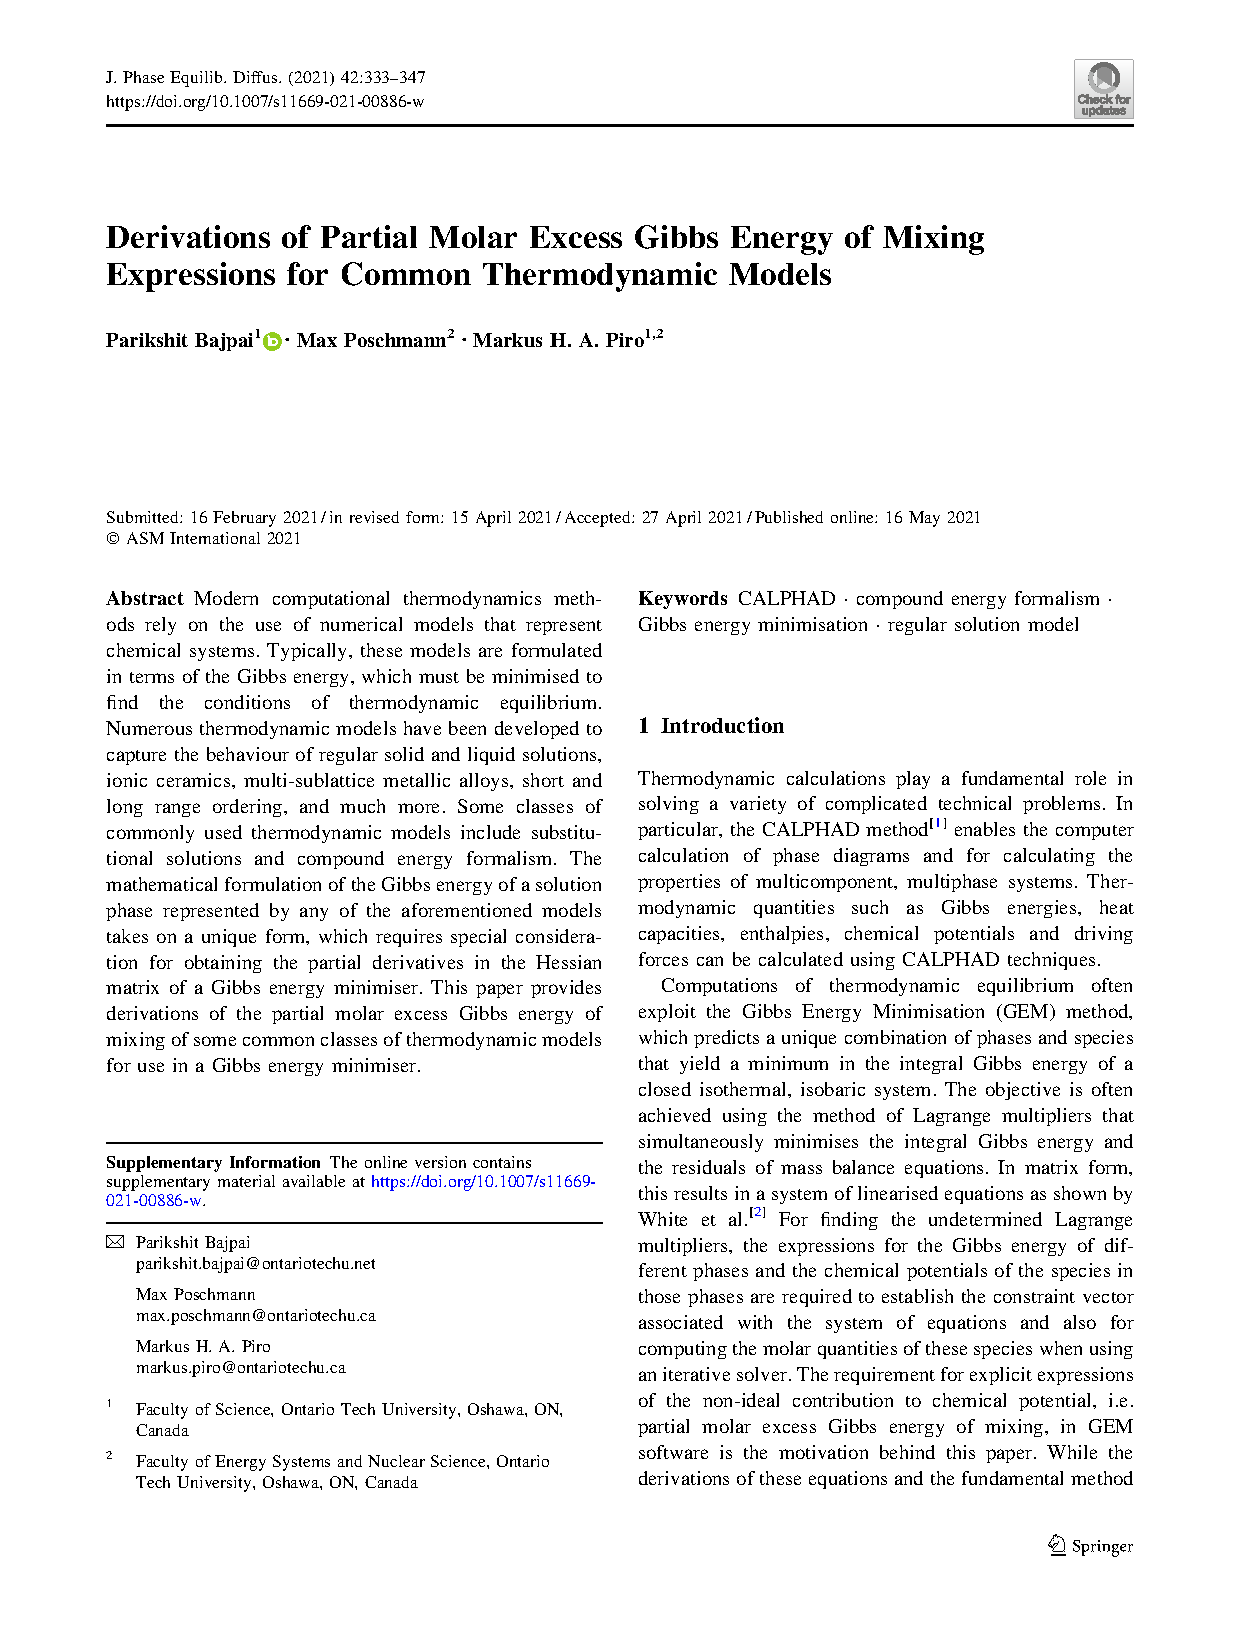
\includepdf[pages=-]{publications/Bajpai_2021_JPED.pdf}
	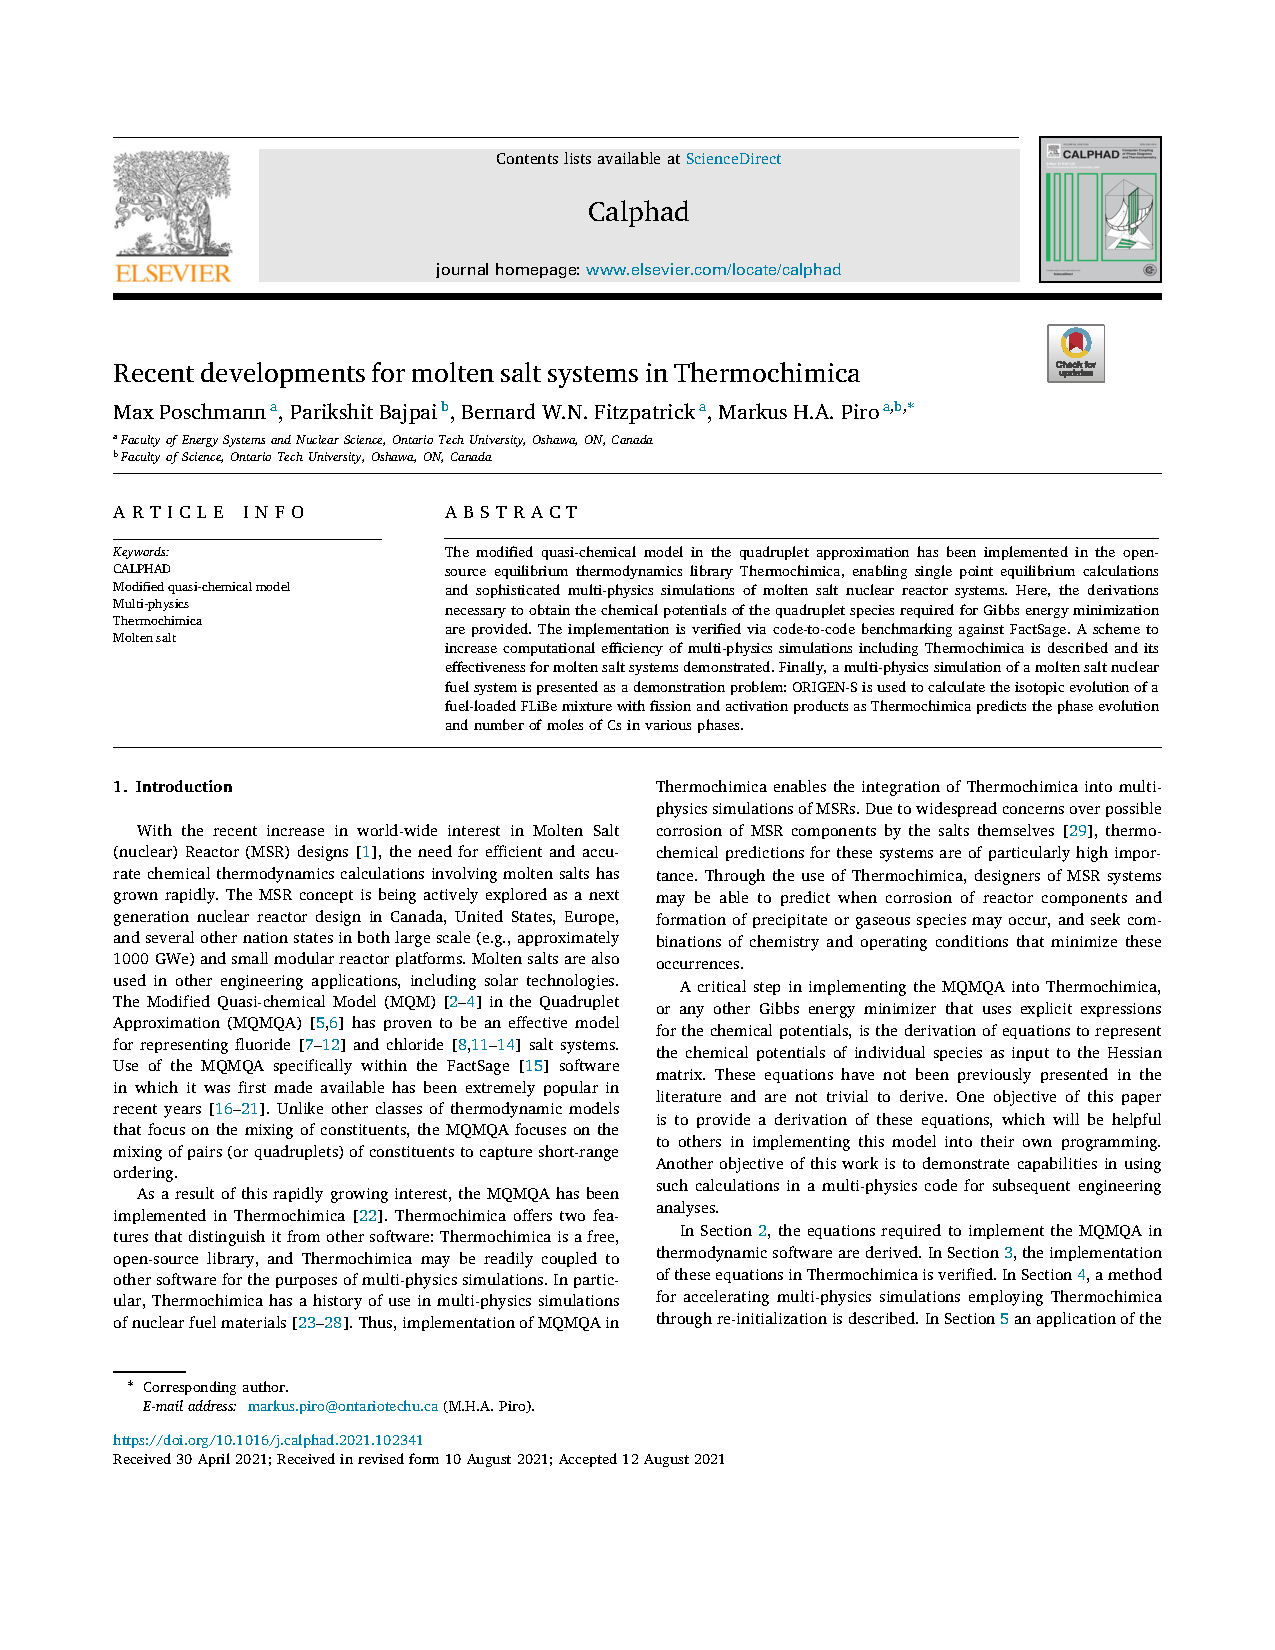
\includepdf[pages=-]{publications/Poschmann_2021_abridged.pdf}
